\documentclass[a4paper,10pt]{report}
\usepackage[utf8]{inputenc}
\usepackage[pdftex]{graphicx}
\usepackage{fancyhdr}
\usepackage{listings}
\usepackage[francais]{babel}
\usepackage{hyperref}
\usepackage{amsmath}

% Title Page
\title{IA01 : TP2}
\author{Par Camille Gerin-Roze et Thomas Perrin}



\renewcommand{\footrulewidth}{1pt}
\fancyfoot[C]{\textbf{\thepage}} 	
\fancyfoot[L]{}

\hypersetup{
	colorlinks=true,
	linkcolor=black
}

\begin{document}

\begin{titlepage}

\begin{flushright}
  
\includegraphics[scale = 0.2]{logo_utc.jpg}
\end{flushright}
\vspace*{5cm}

\newcommand{\HRule}{\rule{\linewidth}{0.5mm}} % Defines a new command for the horizontal lines, change thickness here
\center % Center everything on the page
 


%----------------------------------------------------------------------------------------
%	TITLE SECTION
%----------------------------------------------------------------------------------------

\HRule \\[0.4cm]
{ \LARGE \bfseries  IA01 : Rapport du TP2}\\[0.4cm] % Title of your document
\HRule \\[1.5cm]
 
%----------------------------------------------------------------------------------------
%	AUTHOR SECTION
%----------------------------------------------------------------------------------------
\begin{minipage}{0.4\textwidth}
\begin{flushleft} \large
\emph{Auteurs:}\\
Camille \textsc{Gerin-Roze} \newline
Thomas \textsc{Perrin} 
\end{flushleft}
\end{minipage}
~
\begin{minipage}{0.4\textwidth}

\end{minipage}\\[1.3cm]


{\large Le 15 Novembre 2015} % Date, change the \today to a set date if you want to be precise

\end{titlepage}
\tableofcontents
\chapter*{Introduction}

Le but de ce TP est de réfléchir à une recherche dans un espace d’états avec le langage Lisp. Au départ, nous effectuerons une recherche basique en profondeur,
pour ensuite considérer une heuristique afin d'optimiser cette recherche. 
Dans ce rapport, nous répondrons aux différentes questions posés et nous expliquerons de quel manière nous avons abordé les problèmes et pourquoi.
Nous utiliserons plusieurs fonctions dites « de service » :

\begin{itemize}
 \item get\_symbol : Permet d'obtenir le symbole à l'index en paramètre.
 \item myMember : Implémentation différente de la fonction member avec la fonction EQUAL au lieu de EQ.
 \item etat\_correct : Permet de déterminer si un état est correct en vérifiant la présence de A, B, C, D, que la structure soit de taille 4 et que A soit placé avant D.
 \end{itemize}



\chapter{Graphe d'états}

\begin{figure}[h!]
  \centering
 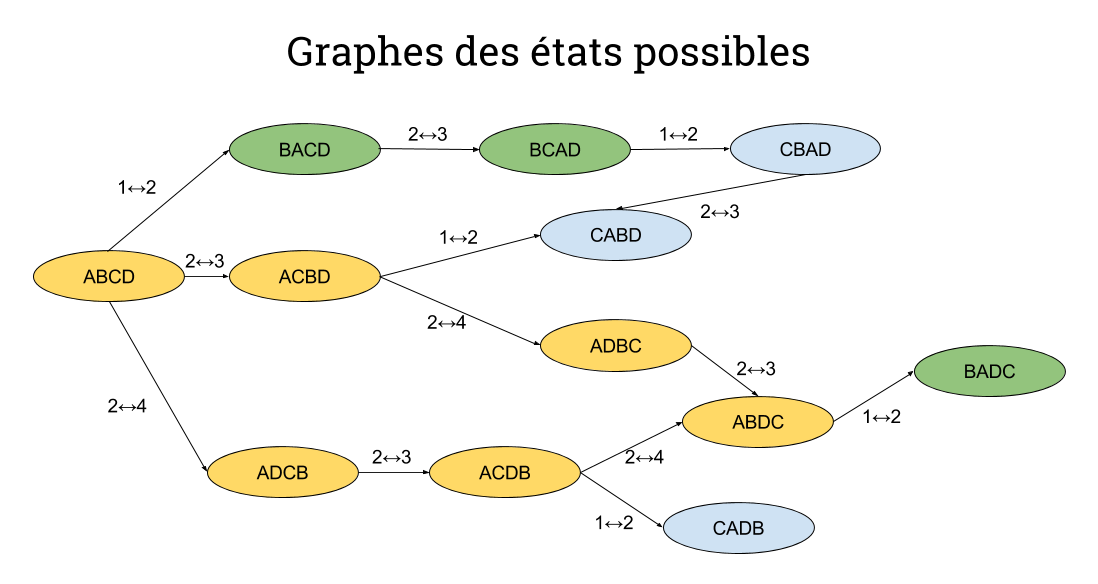
\includegraphics[scale=0.4]{Graphe_D_Etat.png}
 \caption{Graphe représentants les états et leurs successeurs}
\end{figure}

De base, seules trois actions sont possibles à chaque état. Ensuite, à chaque successeur, on retire la même action qui va uniquement revenir en arrière. De plus, certaines actions peuvent être interdites puisqu’ils modifieraient les pions dans un état non autorisé. Ainsi, ce graphe d’états permet de représenter clairement les différentes possibilités en indiquant unitairement chaque état.

\chapter{Développement de l'algorithme de recherche}

  \section{La fonction echange(x,y)}
  La fonction echange reforme les 4 pions à partir d’une liste vide. A chaque itération, on ajoute le pion correspondant, mis à part lorsque l’on est aux deux index précisés en paramètre.  On vérifie ici uniquement que les deux index sont accessibles, on limitera les actions possibles dans la fonction successeurs.
  
  \begin{lstlisting}[language=Lisp]
   
(defun echange(etat x y)
  (if (AND (> x 0) (> y 0) (< x 5) (< y 5))
    (let ((value ()))
      (dotimes (i 5 value)
	(cond
	    ;;;; Si le symbole est x alors on met y
	  ((= i x) (setq value (append value (list (get_symbol etat y)))))
	    ;;;; Si le symbole est y alors on met x
	  ((= i y) (setq value (append value (list (get_symbol etat x))))) 
	    ;;;; Sinon on met le bon symbole
	  ((> i 0) (setq value (append value (list (get_symbol etat i)))))
	)
      )
    )
    ;;;; Gestion des erreurs potentielles
  (error "Les pièces sont positionnées entre 1 et 4")) 
)

  \end{lstlisting}
\newpage
  \section{La fonction successeurs}
  La fonction successeurs effectue les trois actions autorisés par l’énoncé sur l’état en paramètre : c’est-à-dire echange(1,2), echange(2,3) et echange(2,4). Si le successeur est valide (vérifié grâce à la fonction de service etat\_correct), on l’ajoute à la liste des successeurs. Ainsi, on obtiendra une liste pouvant aller de 0 à 3 états.
  \begin{lstlisting}[language=Lisp]
   
(defun successeurs (etat)
  (let ((value ()))
  ;;;; On fait les échanges 1 <-> 2, 2 <-> 3 et 2 <-> 4
  (loop for i in (list 1 3 4) 
    do (if (etat_correct (echange etat i 2))
	    (push (echange etat i 2) value)))
	value)
  )

  \end{lstlisting}
  
  La fonction etat\_correct qui est utilisée sert tout simplement à vérifier qu'un état est correct. On la définie de la façon suivante : 
  \begin{lstlisting}[language=Lisp]
   
(defun etat_correct(e) ;;;; Un etat est correct si 
  (if (AND   ;;;; A est avant D 
	(> (list-length (member 'A e)) (list-length (member 'D e))) 
	(= (list-length e) 4)  ;;;; Si l'etat comporte exactement 4 symboles
	(member 'A e)          ;;;; Si A est membre de l'etat
	(member 'B e)          ;;;; Si B est membre de l'etat
	(member 'C e)          ;;;; Si C est membre de l'etat
	(member 'D e)) T NIL)) ;;;; Si D est membre de l'etat

  \end{lstlisting}

  
  
  
  \newpage
  \section{Algorithme de recherche en profondeur}

   Voici l’algorithme que nous avons développé :
   
   \begin{lstlisting}[basicstyle=\small]
   
fonction Recherche(etatCourant etatFinal etatsParcourus)
	Si (etatCourant = etatFinal) alors
		retourner append(etatsParcourus,etatCourant)
	sinon
		list-succ <- successeurs(etatCourant)
		solution <- NIL
		i <- 0
		Tant que solution = NIL et i < list-length(list-succ)
			Si !membre(list-succ[i], etatsParcourus) alors

			  solution = 
			  Recherche(list-succ[i], etatFinal, 
			    append(etatsParcourus,etatCourant))

			FinSi
			i <- i + 1
		FinTantQue
	FinSi
	
	retourner solution
finRecherche
  \end{lstlisting}

  Cet algorithme permet de tester toutes les solutions en recherchant en profondeur dans l’ensemble d’états. Ainsi, on retombera sur l’état final obligatoirement. Cependant cela peut prendre un certain temps puisque l’algorithme va tester toutes les solutions jusqu’à trouver la bonne. La fonction recherche implémente cet algorithme en plus de rajouter un affichage.
  
  \newpage 
  \section{Implémentation en Lisp de l'algorithme}
  
  \begin{lstlisting}[language=Lisp]
(DEFUN recherche ( etatCourrant etatFinal &optional etatsParcourus)   
  (dotimes (i (list-length etatsParcourus)) 
    (format t "~T"))                         
  (format t "~A~%" etatCourrant)     
  (IF (EQUAL etatCourrant etatFinal)
      (append etatsParcourus (list etatCourrant))      
      (LET ((list-succ (successeurs etatCourrant)) (sol nil))  
	(DO ((succ (pop list-succ) (pop list-succ))) 
	    ((OR (null succ) (not (null sol))) sol) 
	  (IF (AND (NOT (myMember succ etatsParcourus)) (not (null succ))) 
	      (SETQ sol 
		(recherche succ etatFinal 
		    (append etatsParcourus (list etatCourrant)))) 
	      )
	  )
	)
      )
  )
  
    \end{lstlisting}
  
  Cette implémentation est simple : On va dans un premier temps afficher le chemin qui est parcouru, puis  on va vérifier que nous n'avons pas fini notre recherche ( dans ce cas nous sortons de l'algorithme ).
  En suite, pour chaque successeurs valide, nous allons rappeller notre fonction récursivement, de manière à continuer notre recherche avec chaque successeur de notre 
  état initial.

  Voici l’appel de la fonction recherche :
  \begin{lstlisting}[language=Lisp]
(recherche '(A D B C) '(C B A D))
(A D B C)
 (A C B D)
  (A B C D)
   (A D C B)
    (A C D B)
     (A B D C)
      (B A D C)
     (C A D B)
   (B A C D)
    (B C A D)
     (C B A D)
((A D B C) (A C B D) (A B C D) (B A C D) (B C A D) (C B A D))
  \end{lstlisting}

On peut observer que l’algorithme trouve le chemin comme prévu. 
Cependant, on peut remarquer qu’il remonte dans ses appels trois fois avant de trouver le bon chemin et que le chemin est loin d'être optimal.

\chapter{Rechercher avec une heuristique}

  \section{Déterminer une heuristique}
  L’ajout d’une heuristique permettra de choisir l’état d’une manière plus cohérente pour continuer les itérations. Nous avons choisi d’utiliser la distance entre chaque état afin de déterminer lequel est le plus proche de l’état final. La distance est caractérisée par la différence entre chaque lettre entre deux états. Par exemple, ABCD et ABDC ont une distance de 2 car deux lettres sont interverties. 
Ainsi, si nous avons le choix entre un état possédant une seule différence avec l’état final ou un second trois différences avec ce dernier, on choisira le premier état.
Afin d’obtenir un résultat plus pertinent, nous ne regarderons pas le deuxième symbole puisque ce dernier bougera constamment.\newline
En effet, chaque action possible demande de déplacer le deuxième symbole, donc quand deux états ont la même distance, si un des deux états a son deuxième symbole bien placé
alors l'autre sera plus proche de l'état final. Prenons un exemple avec l'état ABCD : \newline
Prenons l'exemple de ABDC et ACBD, ces deux états sont à une distance de deux symboles avec ABCD ( ils ont deux symboles différents ). Cependant, il faut une seule opération
sur ACBD pour arriver à ABCD ( echange(2,3) ) tandis qu'il faut au minimum 3 opérations à ABDC pour atteindre ABCD. C'est parce que dans les symboles bien placés de 
ABDC, il y a le deuxième symbole qui sera forcément changé quand nous bougerons les autres symboles.\newline
Donc nous choisissons de calculer la distance entre deux états en omettant volontairement le deuxième symbole.
La fonction distance permet de calculer la distance entre deux états et permet de représenter cette heuristique.
Notre heuristique peut donc être résumé en la phrase :
`` Un état est estimé plus proche de l'état final si la distance ométtant le deuxième symbole entre celui-ci et l'état final est minimale.''\newpage 
  \section{Implémentation de la distance}

  \begin{lstlisting}[language=Lisp]
   (defun distance (etatA etatB)
  (let ((dist 0) (x (pop etatA)) (y (pop etatB)))
    (loop for i from 0 to 4 do
	  (if (AND (NOT (= i 1))(NOT (EQUAL x y)))
	      (setq dist (1+ dist)))
	  (setq x (pop etatA))
	  (setq y (pop etatB))
	  )
    dist
    )
  )
  \end{lstlisting}
  \section{Implémentation du choix de l'état}

    \begin{lstlisting}[language=Lisp]

  (defun choixEtat (etat liste parcouru)
  (let ((minDist)(minEtat))
    (dolist (e liste minEtat)
      (if (AND ;;;; Si la distance entre e et minEtat est plus petite
	   (OR (AND (NULL minDist) (NULL minEtat)) 
		    (< (distance etat e) minDist)) 
	   ;;;; ET si e n'a pas déja été parcouru
	   (NOT (MYMEMBER e parcouru)))        
	  (progn
	  ;;;; ALORS e est un état plus prometteur que minEtat
	    (setq minDist (distance etat e))   
	    (setq minEtat e)
	    )
	)
      )
    minEtat ;;;; On retourne le meilleur état trouvé
    )
  )
  \end{lstlisting}

\newpage
  
  \section{Implémentation de notre nouvelle fonction de recherche}
  
  Notre nouvelle fonction de recherche va donc utiliser notre heuristique par le biais de la fonction choixEtat. 
  Pour cela, la fonction recherche\_opti va appeller la fonction choix etat pour que celle-ci trouve l'état le plus prometteur, si cet 
  état ne donne pas de solution alors on rapellera la fonction choix état pour qu'elle nous donne le deuxième état le plus prometteur et 
  cela jusqu'à ce qu'il y ai une solution ou qu'il n'y ai plus de successeurs.\newline Cela nous donne l'implémentation suivante : 
  
  \begin{lstlisting}[basicstyle = \footnotesize, language=Lisp]
    (DEFUN recherche_opti ( etatCourrant etatFinal &optional etatsParcourus)
  (if (NOT (AND (etat_correct etatCourrant) (etat_correct etatFinal)))
      (error "ERREUR : ENTREE(S) INCORRECT(S)")
      )
  (dotimes (i (list-length etatsParcourus))
    (format t "~T"))                       
  (format t "~A~%" etatCourrant)            
  (IF (EQUAL etatCourrant etatFinal)
      (append etatsParcourus (list etatCourrant))
	  (let (
	  (etatPrometteur (choixEtat etatFinal (successeurs etatCourrant) etatsParcourus))
	  )
      	(loop while (not (null etatPrometteur))
	      do 
	      (if (NOT (MYMEMBER etatPrometteur etatsParcourus)) 
			  (SETQ 
			  sol (recherche_opti etatPrometteur etatFinal 
				  (append etatsParcourus (list etatCourrant)))
			  )
			)
			(if (null sol)
				(setq etatPrometteur 
				    (choixEtat etatFinal (remove etatPrometteur 
					  (successeurs etatCourrant)) etatsParcourus))
				(setq etatPrometteur NIL)
			)
		 )
    sol)
  )
 )
 
  \end{lstlisting}
\newpage 
  \section{Comparaison des fonctions avec et sans heuristique }
  
  Voici l’appel de la fonction recherche\_opti :
\begin{lstlisting}[language=Lisp]
(recherche_opti '(A D B C) '(C B A D))
(A D B C)
 (A C B D)
  (C A B D)
   (C B A D)
((A D B C) (A C B D) (C A B D) (C B A D))
\end{lstlisting}

On remarque que le chemin retourné par notre heuristique est plus court que celui utilisé retourné par une recherche basique en profondeur.
Ainsi, lorsque l’on analyse le problème, et que l’on sait comment se rapprocher de la solution en simplifiant une recherche, on peut voir que l’on gagne du temps en termes de parcours. La complexité à chaque itération est plus élevée puisqu’il faut comparer les prédécesseurs avant de continuer. Mais cette analyse est moins couteuse que d’itérer pour rien sur certains états par la suite.

On peut conclure qu’une heuristique est très avantageuse en termes de performance et de qualité de résultats. Sur des applications de recherche à plus grande envergures tels que la recherche de chemin dans des réseaux, les heuristiques sont obligatoires afin d’obtenir des performances convenables.

\chapter*{Conclusion}

  La recherche dans un espace d'état peut effectivement être faite de manière naïve en parcourant l'arbre bêtement en profondeur ou en largeur. Mais on s'aperçoit
  que l'utilisation d'une heuristique peut permettre d'une part, d'avoir des résultats bien plus intéressant, et d'autre part, d'accélérer le traitement de certaines 
  requêtes en diminuant de manière significative le nombre d'itération de la boucle principale. \newline 
  Cependant, on pourra noter qu'une heuristique n'est pas toujours bénéfique dans tous les cas. En effet dans le choix des etats, choisir l'état le plus proche de 
  l'état final ne sera pas toujours le chemin le plus court et un algorithme de recherche naïf pourrait trouver un meilleur résultat par pure hasard.
  
  \end{document}          


